\section{A finite-volume criterion for the full gap}
\label{sec:finite-volume}

We first isolate a finite-volume statement that will be sufficient for a
mass gap. It involves the actual partition functions, so it sees every
spectral sector. It is also insensitive to a contribution to the free
energy proportional to volume, which will make it suitable for
renormalization.

\subsection{Transfer eigenvalues and a measure of excited-state weight}

Fix a spatial circumference \(w\). A time slice is a configuration
\(s=(s_1,\ldots,s_w)\in(S^3)^w\). Set
\(V_w(s)=\sum_{i=1}^w s_i\cdot s_{i+1}\), with periodic indices, and let
\(K_w\) be the integral operator with kernel
\begin{equation}
\label{eq:transfer-kernel}
 K_w(s,s')=
 \exp\!\left[\frac\beta2 V_w(s)+\beta\sum_{i=1}^w s_i\cdot s'_i
                         +\frac\beta2V_w(s')\right].
\end{equation}
The operator is compact and self-adjoint. It is positive semidefinite:
the expansion of \(e^{\beta s\cdot s'}\) is a sum of positive
tensor-product kernels, and multiplication on both sides by
\(e^{\beta V_w/2}\) preserves positivity. The positive-kernel series has
finite diagonal integral, so it also proves trace class. The strictly
positive kernel gives a simple largest eigenvalue. Write
\(\lambda_1(w)>\lambda_2(w)\ge\lambda_3(w)\ge\cdots\ge0\), allowing
\(\lambda_2=0\). Closing the time direction gives
\begin{equation}
\label{eq:trace}
 Z_\beta(n,w)=\Tr K_w^n=\sum_i\lambda_i(w)^n.
\end{equation}

Suppress \(\beta\) temporarily and define
\begin{align}
 p(n,w)&=2\log Z(n,w)-\log Z(2n,w),\label{eq:p}\\
 q(n,w)&=2\log Z(n,w)-\log Z(n,2w).\label{eq:q}
\end{align}
Both are nonnegative. To interpret \(p\), introduce the normalized trace
weights
\begin{equation}
 t_i=\frac{\lambda_i(w)^n}{\sum_j\lambda_j(w)^n}.
 \qquad\text{Then}\qquad
 e^{-p(n,w)}=\sum_i t_i^2.
\label{eq:purity}
\end{equation}
Thus small \(p\) means that almost all the trace weight lies in one
eigenstate, necessarily the ground state. The same interpretation applies
to \(q\) after interchanging the coordinate directions.

\begin{samepage}
\begin{lemma}
\label{lem:squaring}
The excited trace tail
\[
 s_n(w)=\sum_{i\ge2}\left(\frac{\lambda_i(w)}{\lambda_1(w)}\right)^n
\]
satisfies \(s_n(w)\le e^{p(n,w)}-1\). If \(p(n,w)\le1/4\), then
\begin{equation}
\label{eq:squaring}
 \left(\frac{\lambda_2(w)}{\lambda_1(w)}\right)^n\le2p(n,w),
 \qquad p(2n,w)\le4p(n,w)^2.
\end{equation}
The analogous statements hold for \(q\) when the other period is doubled.
\end{lemma}
\end{samepage}

\begin{proof}
Since \(\sum_i t_i^2\le t_1=(1+s_n)^{-1}\), we have
\(s_n\le e^p-1\). For \(p\le1/4\), this is at most \(pe^p\le2p\),
which also bounds the first excited term. The largest eigenvalue cancels
from the definition of \(p\), so
\[
 p(2n,w)=2\log(1+s_{2n})-\log(1+s_{4n})
 \le2s_{2n}\le2s_n^2\le2p^2e^{2p}\le4p^2.
\]
\end{proof}

\subsection{Increasing the spatial volume}

Ground-state dominance at one fixed circumference is not enough. New
low-energy states could appear as the circumference increases. The
following exact identity lets us control that limit:
\begin{equation}
\label{eq:rectangle}
 p(n,2w)=2p(n,w)-2q(n,w)+q(2n,w).
\end{equation}
It follows by substituting \eqref{eq:p}--\eqref{eq:q}. There is a second
identity obtained by interchanging the directions.

Figure~\ref{fig:rectangle-doubling} records the two-direction geometry.
\begin{figure}[tbp]
  \centering
  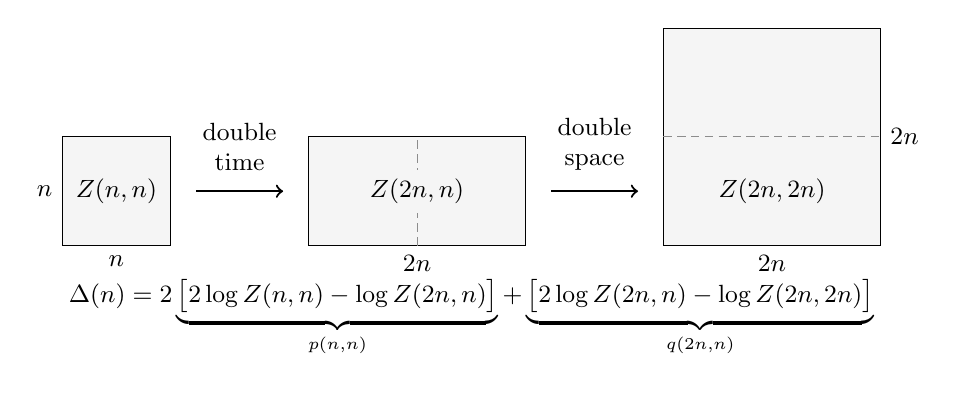
\begin{tikzpicture}[x=0.92cm,y=0.92cm,font=\small]
    \draw[fill=black!4] (0,0) rectangle (1.5,1.5);
    \node at (0.75,0.75) {$Z(n,n)$};
    \node[below] at (0.75,0) {$n$};
    \node[left] at (0,0.75) {$n$};

    \draw[->,thick] (1.85,0.75) -- (3.05,0.75);
    \node[align=center,above] at (2.45,0.9) {double\\time};

    \draw[fill=black!4] (3.4,0) rectangle (6.4,1.5);
    \draw[densely dashed,black!45] (4.9,0) -- (4.9,1.5);
    \node[fill=black!4] at (4.9,0.75) {$Z(2n,n)$};
    \node[below] at (4.9,0) {$2n$};

    \draw[->,thick] (6.75,0.75) -- (7.95,0.75);
    \node[align=center,above] at (7.35,0.9) {double\\space};

    \draw[fill=black!4] (8.3,0) rectangle (11.3,3);
    \draw[densely dashed,black!45] (8.3,1.5) -- (11.3,1.5);
    \node at (9.8,0.75) {$Z(2n,2n)$};
    \node[below] at (9.8,0) {$2n$};
    \node[right] at (11.3,1.5) {$2n$};

    \node at (5.65,-1.0)
      {$\displaystyle
        \Delta(n)=2\underbrace{\bigl[2\log Z(n,n)-\log Z(2n,n)\bigr]}_{p(n,n)}
          +\underbrace{\bigl[2\log Z(2n,n)-\log Z(2n,2n)\bigr]}_{q(2n,n)}$};
  \end{tikzpicture}\par\medskip
  \caption{The two coordinate directions enter the square-box test.
  Every rectangle has periodic boundary conditions; the dashed lines
  mark its dimensions, not cuts that make the pieces independent.
  The second doubling starts from the enlarged rectangle.
  The displayed identity is exact, with the fixed coupling suppressed.}
  \label{fig:rectangle-doubling}
\end{figure}


Define the square-box test
\begin{equation}
\label{eq:Delta}
 \Delta_\beta(n)=4\log Z_\beta(n,n)-\log Z_\beta(2n,2n).
\end{equation}
It obeys
\(\Delta_\beta(n)=2p(n,n)+q(2n,n)\ge0\). The coefficients in
\eqref{eq:Delta} cancel any term proportional to the area of the box.

\begin{samepage}
\begin{proposition}[Finite-volume criterion]
\label{prop:criterion}
Let \(n\ge4\) be even. If
\begin{equation}
 \Delta_\beta(n)\le\eta_*:=2^{-10},
\label{eq:small-test}
\end{equation}
then the transfer operators on circumferences \(2^kn\), \(k\ge0\), satisfy
\begin{equation}
 \frac{\lambda_2(2^kn)}{\lambda_1(2^kn)}
 \le e^{-(\log2)/n}.
\label{eq:width-gap}
\end{equation}
Every local limit of the square tori with sides \(2^kn\) has full gap
at least \((\log2)/n\). In particular, if the periodic infinite-plane
state is unique, then
\begin{equation}
\label{eq:criterion-gap}
 \gap(\beta)\ge\frac{\log2}{n}.
\end{equation}
\end{proposition}
\end{samepage}

\begin{proof}
Write \(\Delta=\Delta_\beta(r)\). Besides
\(q(2r,r)\le\Delta\), the definitions give
\(p(r,2r)=\Delta-2q(r,r)\le\Delta\).
Lemma~\ref{lem:squaring} therefore yields
\(p(2r,2r)\le4\Delta^2\). The rectangle identity in the other direction
gives
\[
 q(4r,r)=2q(2r,r)-2p(2r,r)+p(2r,2r)
 \le2\Delta+4\Delta^2\le3\Delta.
\]
Squaring in that direction gives \(q(4r,2r)\le36\Delta^2\). Consequently,
\begin{equation}
 \Delta_\beta(2r)
 =2p(2r,2r)+q(4r,2r)
 \le44\Delta_\beta(r)^2\le64\Delta_\beta(r)^2.
\label{eq:quadratic-recursion}
\end{equation}
Every use of the lemma is justified by \(3\eta_*<1/4\), and the smallness
condition is preserved. For \(n_k=2^kn\), induction gives
\[
 \Delta_\beta(n_k)\le\frac1{64}
          (64\eta_*)^{2^k}\le\frac1{64}2^{-2^k}.
\]
Since the first assertion of the lemma bounds
\((\lambda_2(n_k)/\lambda_1(n_k))^{n_k}\) by
\(2p(n_k,n_k)\le\Delta_\beta(n_k)\), taking the \(n_k\)-th root proves
\eqref{eq:width-gap}.

Let \(\Omega_w\) be the normalized positive ground eigenvector of
\(K_w\). For a bounded continuous observable \(F\) supported in a time slab of finite
thickness, let \(K_{w,F}\) denote the transfer kernel across that slab
with the insertion of \(F\). Pointwise,
\(|K_{w,F}|\le\norm{F}_\infty K_w^r\), where \(r\) is the number of
transfer steps across the slab. Set \(A_F=K_{w,F}/\lambda_1(w)^r\);
for \(r=0\), this is multiplication by \(F\).
Its operator norm is at most \(\norm{F}_\infty\). The infinite-time
cylinder expectation is
\(\omega_w(F)=\inner{\Omega_w}{A_F\Omega_w}\). Applying
\eqref{eq:width-gap} between two such insertions gives
\begin{equation}
 |\Cov_{\omega_w}(F,G)|\le\norm{F}_\infty\norm{G}_\infty
                           e^{-(\log2)d/n},
\label{eq:slab-bound}
\end{equation}
where \(d\) is the number of transfer edges separating their supports.
This bound passes to any local limit of the cylinder states as
\(w=2^kn\to\infty\).

We can identify these limits directly with the square-torus limits.
Let \(\widehat K_w=K_w/\lambda_1(w)\). If \(w=n_k\) and \(r\le w/2\), the
square-torus expectation is
\[
 \frac{\Tr(A_F\widehat K_w^{\,w-r})}{\Tr\widehat K_w^{\,w}}.
\]
Separating the ground projection in numerator and denominator shows that
its difference from the cylinder expectation is at most
\(2\norm{F}_\infty s_{w/2}(w)\). But
\[
 p(w/2,w)\le\Delta_\beta(w/2),\qquad
 s_{w/2}(w)\le e^{\Delta_\beta(w/2)}-1\longrightarrow0.
\]
Thus the square and cylinder expectations have the same subsequential
limits, also for products of fixed local observables. In particular,
\eqref{eq:slab-bound} holds in every such square-torus limit.

For each centered vector created by a local observable in the
reflection-positive Hilbert space, the transfer autocorrelation has a
positive spectral measure. It is a correlation of two reflected slabs,
so \eqref{eq:slab-bound} applies and excludes spectral support above
\(e^{-(\log2)/n}\) for that vector. Such vectors are dense in the vacuum
orthogonal subspace, so the same exclusion holds for the full transfer
operator. This proves \eqref{eq:criterion-gap}.
\end{proof}

The slab estimate extends to bounded measurable local observables by
approximation in their finite-dimensional distributions. No prefactor
depending on the size of a slab is needed; this will be useful for the
upper mass bound.

The criterion has reduced the problem to a single question: can one make
\(\Delta_\beta(n)\) small with \(n\) no larger than a fixed multiple of
\(\rho(\beta)^{-1}\)? The preliminary estimate alone will not do this.
It will instead supply a reference box for the comparison between cutoffs.


